    \subsection{Audit of the Smart Contracts}
        The objective of this subsection is to perform a security analysis of the Smart Contracts from the  \acrshort{mvp}1 in order to detect vulnerabilities, with the aim of improving the quality of the Contracts.\\
        
        For this purpose, two analyses will be made. One with the tool \textit{Mythril}\footnote{\url{https://github.com/ConsenSys/mythril}}. \textit{Mythril} (figure \ref{fig:myth}) is a security analysis tool for \acrshort{evm} bytecode. It detects security vulnerabilities in Smart Contracts built for \textit{Ethereum}, \textit{Hedera}, \textit{Quorum}, \textit{Vechain}, \textit{Roostock}, \textit{Tron} and other \acrshort{evm}-compatible blockchains. It uses symbolic execution, \acrshort{smt} solving and taint analysis to detect a variety of security vulnerabilities.
        \begin{figure}[h]
            \centering
            \includegraphics[width=0.3\textwidth]{mythril_logo.png}
            \caption{Mythril logo}
            \label{fig:myth}
        \end{figure}
        
        In addition, a dead code analysis will be done, to detect failures in the code of the Smart Contracts.
        
        \subsubsection{Mythril analysis}
            In the \acrshort{mvp}1 of Alastria ID, eight Smart Contracts have been designed and two libraries have been used.\\
            
            To facilitate the audit, some scripts have been designed in \textit{Shell Script}. The first script called \textit{audit.sh} (listing \ref{lst:audit.sh}) performs the analysis with the \textit{Mythril} tool. A docker container has been created for each contract and the analysis has been carried out in this container. This analysis has been programmed to last a maximum of two hours.
        
            \lstinputlisting[label={lst:audit.sh}, caption=audit.sh source code, language=bash]{examples/mythrilAudit/audit.sh}
        
            In order to obtain the reports after the completion of \textit{audit.sh}, another script has been made, called \textit{getReports.sh} (listing \ref{lst:getReports.sh}). This script copies the logs of the different containers created into different files, so that they are more comfortable to handle and read.\\
            
            \lstinputlisting[label={lst:getReports.sh}, caption=getReports.sh source code, language=bash]{examples/mythrilAudit/getReports.sh}
            
            After the analysis, and the study of the reports, the following results have been obtained:
            \paragraph{AlastriaCredentialRegistry.sol}
                The following table (table \ref{tab:AlastriaCredentialRegistry}) summarizes the vulnerabilities found in the Smart Contract \textit{AlastriaCredentialRegistry}.
                \begin{longtable}{||p{0.1\linewidth} | p{0.11\linewidth} | p{0.52\linewidth} | p{0.3\linewidth}||}
                    \hline
                    \textbf{\acrshort{swc} ID} & \textbf{Severity} & \textbf{Functions} & \textbf{Description} \\ [0.5ex] 
                    \hline\hline
                    \href{https://swcregistry.io/docs/SWC-101}{101} & High & addSubjectCredential (bytes32, string) & The arithmetic operator can overflow.\\ 
                    \hline
                    \href{https://swcregistry.io/docs/SWC-110}{110} & Medium & issuerCredentialList (address, uint256) & An assertion violation was triggered.\\
                    \cline{3-3}
                    & & getCredentialStatus (uint8, uint8) &\\ 
                    \cline{3-3} 
                    & & subjectCredentialList (address, uint256) &\\
                    \cline{3-3}
                    & & updateCredentialStatus (bytes32, uint8) &\\ [1ex] 
                    \hline
                    \caption{AlastriaCredentialRegistry.sol Mythrill audit report}
                    \label{tab:AlastriaCredentialRegistry}
                \end{longtable}

            \newpage

            \paragraph{AlastriaIdentityEntity.sol}
                The following table (table \ref{tab:AlastriaIdentityEntity}) summarizes the vulnerabilities found in the Smart Contract \textit{AlastriaIdentityEntity}.
                \begin{longtable}{||p{0.1\linewidth} | p{0.11\linewidth} | p{0.5\linewidth} | p{0.3\linewidth}||}
                    \hline
                    \textbf{\acrshort{swc} ID} & \textbf{Severity} & \textbf{Functions} & \textbf{Description} \\ [0.5ex] 
                    \hline\hline
                    \href{https://swcregistry.io/docs/SWC-101}{101} & High & setUrlLogo (address, string) & The arithmetic operator can overflow. \\
                    \cline{3-3}
                    & & setCifEntity (address, string)  &\\
                    \cline{3-3}
                    & & setUrlCreateAID (address, string) &\\
                    \cline{3-3}
                    & & setUrlAOA (address, string) &\\
                    \cline{3-3}
                    & & setNameEntity (address, string) &\\[1ex] 
                    \hline
                    \caption{AlastriaIdentityEntity.sol Mythrill audit report}
                    \label{tab:AlastriaIdentityEntity}
                \end{longtable}
                
            \paragraph{AlastriaIdentityIssuer.sol}
                The following table (table \ref{tab:AlastriaIdentityIssuer}) summarizes the vulnerabilities found in the Smart Contract \textit{AlastriaIdentityIssuer}.
                \begin{longtable}{||p{0.1\linewidth} | p{0.11\linewidth} | p{0.45\linewidth} | p{0.35\linewidth}||}
                    \hline
                    \textbf{\acrshort{swc} ID} & \textbf{Severity} & \textbf{Functions} & \textbf{Description} \\ [0.5ex] 
                    \hline\hline
                    \href{https://swcregistry.io/docs/SWC-107}{107} & Low & updateIdentityIssuerEidasLevel\newline (address, uint8) & Read of persistent state following external call.\\
                    \cline{3-3}
                    & & addIdentityIssuer (address, uint8) &\\[1ex]
                    \hline
                    \href{https://swcregistry.io/docs/SWC-110}{110} & Medium & updateIdentityIssuerEidasLevel\newline (address, uint8) & An assertion violation was triggered.\\
                    \cline{3-3}
                    & & addIdentityIssuer (address, uint8) &\\
                    \cline{3-3}
                    \hline
                    \caption{AlastriaIdentityIssuer.sol Mythrill audit report}
                    \label{tab:AlastriaIdentityIssuer}
                \end{longtable}
                
            \paragraph{AlastriaIdentityManager.sol}
                No vulnerabilities were found in \textit{AlastriaIdentityManager.sol} after the audit.
                
            \paragraph{AlastriaIdentityServiceProvider.sol}
                No vulnerabilities were found in \textit{AlastriaIdentityServiceProvider.sol} after the audit.
                
            \paragraph{AlastriaPresentationRegistry.sol}
                No vulnerabilities were found in \textit{AlastriaPresentationRegistry.sol} after the audit.
                
            \paragraph{AlastriaProxy.sol}
                The following table (table \ref{tab:AlastriaProxy}) summarizes the vulnerabilities found in the Smart Contract \textit{AlastriaIdentityIssuer}.\newline
                \begin{longtable}{||p{0.1\linewidth} | p{0.11\linewidth} | p{0.45\linewidth} | p{0.35\linewidth}||}
                    \hline
                    \textbf{\acrshort{swc} ID} & \textbf{Severity} & \textbf{Functions} & \textbf{Description} \\ [0.5ex] 
                    \hline\hline
                    \href{https://swcregistry.io/docs/SWC-107}{107} & Low & forward (address, uint256, bytes) & A call to a user-supplied address is executed. An external message call to an address specified by the caller is executed.\\ [1ex] 
                    \hline
                    \caption{AlastriaProxy.sol Mythrill audit report}
                    \label{tab:AlastriaProxy}
                \end{longtable}
                
            \paragraph{AlastriaPublicKeyRegistry.sol}
                The following table (table \ref{tab:AlastriaPublicKeyRegistry}) summarizes the vulnerabilities found in the Smart Contract \textit{AlastriaPublicKeyRegistry}.
                \begin{longtable}{||p{0.1\linewidth} | p{0.11\linewidth} | p{0.45\linewidth} | p{0.35\linewidth}||}
                    \hline
                    \textbf{\acrshort{swc} ID} & \textbf{Severity} & \textbf{Functions} & \textbf{Description} \\ [0.5ex] 
                    \hline\hline
                    \href{https://swcregistry.io/docs/SWC-110}{110} & Medium & publicKeyList (address, uint256) & An assertion violation was triggered.\\ [1ex] 
                    \hline
                    \caption{AlastriaPublicKeyRegistry.sol Mythrill audit report}
                    \label{tab:AlastriaPublicKeyRegistry}
                \end{longtable}
        
            \paragraph{Eidas.sol}
                The following table (table \ref{tab:Eidas}) summarizes the vulnerabilities found in the Smart Contract \textit{Eidas}.
                \begin{longtable}{||p{0.1\linewidth} | p{0.11\linewidth} | p{0.50\linewidth} | p{0.30\linewidth}||}
                    \hline
                    \textbf{\acrshort{swc} ID} & \textbf{Severity} & \textbf{Functions} & \textbf{Description} \\ [0.5ex] 
                    \hline\hline
                    \href{https://swcregistry.io/docs/SWC-110}{110} & Medium & atLeast\newline (Eidas.EidasLevel, Eidas.EidasLevel) & An assertion violation was triggered.\\
                    \cline{3-3}
                    & & atLeastLow (Eidas.EidasLevel) &\\[1ex] 
                    \hline
                    \caption{Eidas.sol Mythrill audit report}
                    \label{tab:Eidas}
                \end{longtable}
                
            \paragraph{Owned.sol}
                No vulnerabilities were found in \textit{Owned.sol} after the audit.\\

            \begin{figure}[h]
                \centering
                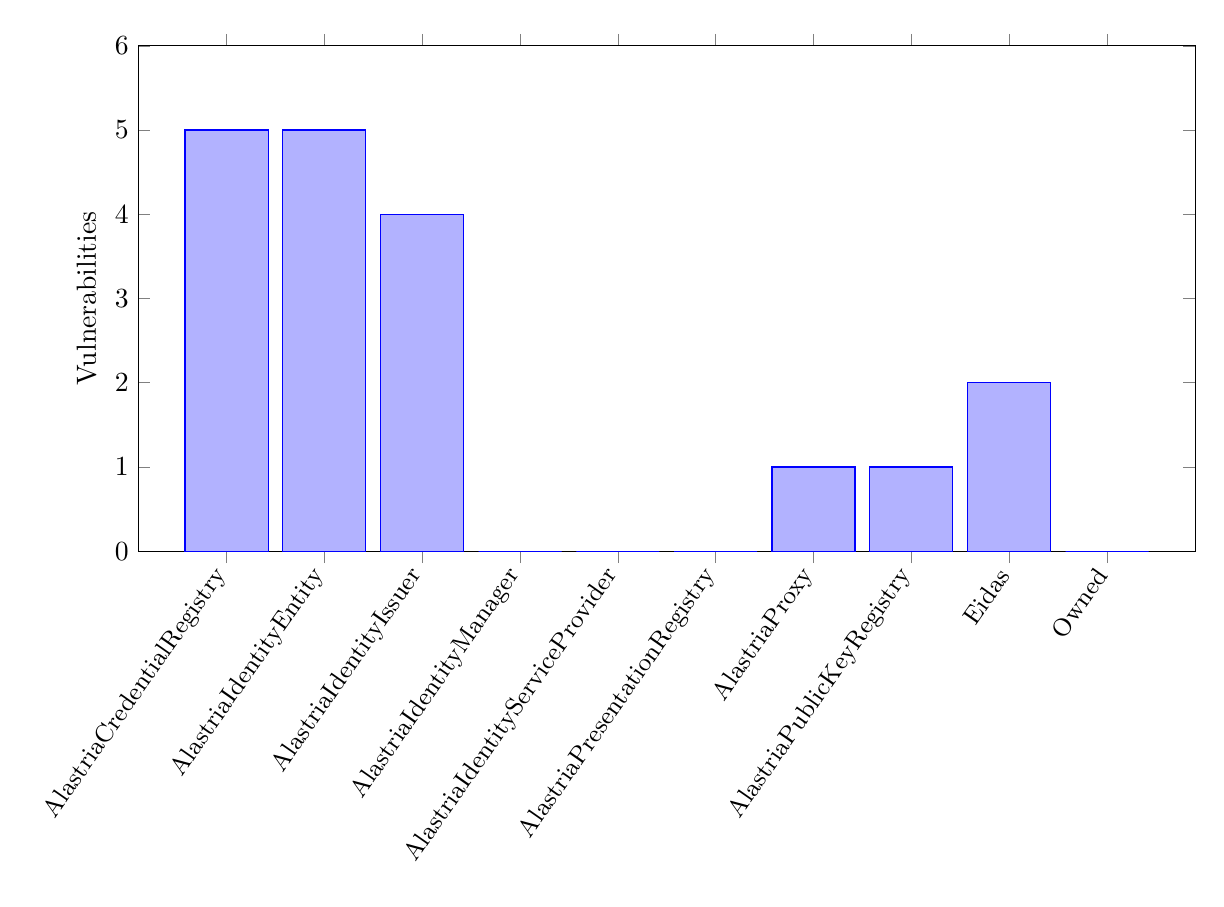
\begin{tikzpicture}
                    \begin{axis}[
                     width=15cm,
                     height=8cm,
                     symbolic x coords={AlastriaCredentialRegistry, AlastriaIdentityEntity, AlastriaIdentityIssuer, AlastriaIdentityManager, AlastriaIdentityServiceProvider, AlastriaPresentationRegistry, AlastriaProxy, AlastriaPublicKeyRegistry, Eidas, Owned},
                     x tick label style={rotate=55, font=\small,anchor=east},
                     xtick=data,
                     ymin=0,
                     ymax=6,
                     ylabel=Vulnerabilities,
                     ybar,
                     bar width=30pt,
                     ]
                    \addplot coordinates {
                        (AlastriaCredentialRegistry, 5)
                        (AlastriaIdentityEntity, 5)
                        (AlastriaIdentityIssuer, 4)
                        (AlastriaIdentityManager, 0)
                        (AlastriaIdentityServiceProvider, 0)
                        (AlastriaPresentationRegistry, 0)
                        (AlastriaProxy, 1)
                        (AlastriaPublicKeyRegistry, 1)
                        (Eidas, 2)
                        (Owned, 0)};
                    \end{axis}
                \end{tikzpicture}
                \caption{Number of vulnerabilities by Smart Contract}
                \label{fig:bars-scs}
            \end{figure}
            
            In conclusion to the analysis, we can see that Smart Contracts \textit{AlastriaCredentialRegistry} and \textit{AlastriaIdentityEntity} are the ones that have found the most vulnerabilities, with five each one (figure \ref{fig:bars-scs}). In relation to the vulnerabilities found, we see that \textbf{33\% (6) are high}, another \textbf{55\% (9) are medium} and \textbf{17\% (3) are low} (figure \ref{fig:pie-scs}).\\
            \begin{figure}[h!]
                \centering
                \begin{tikzpicture}
                    \pie[radius=2]{33/High, 50/Medium, 17/Low}
                \end{tikzpicture}
                \caption{Criticality of the Smart Contracts vulnerabilities}
                \label{fig:pie-scs}
            \end{figure}
        
            Below are some points to mitigate the vulnerabilities found.\\
            
            An \textbf{arithmetic overflow (\acrshort{swc} \href{https://swcregistry.io/docs/SWC-101}{101})} means that it is possible to cause an integer overflow or underflow in an arithmetic operation. This means that you can store in a variable a value larger than its limit. This can be solved by checking if it is possible to overflow or underflow before performing the operation. It is advisable to use standard libraries already defined that mitigate this attack. An example of a standard library is \textit{SafeMath.sol}\footnote{\url{https://github.com/OpenZeppelin/openzeppelin-contracts/blob/master/contracts/math/SafeMath.sol}}, developed by \textit{OpenZeppelin}.\\
            
            In relation to the \textbf{reentrancy (\acrshort{swc} \href{https://swcregistry.io/docs/SWC-107}{107})}, an external message call to an address specified by the caller can be executed. The callee account might contain arbitrary code and could re-enter any function within this contract. Reentering the contract in an intermediate state may lead to unexpected behavior. To mitigate this, you have t make sure that no state modifications are executed after the call and/or reentrancy guards are in place. Also, with this vulnerability, the contract account state is accessed after an external call to a fixed address. To prevent reentrancy issues, consider accessing the state only before the call, especially if the callee is untrusted. Alternatively, a reentrancy lock can be used to prevent untrusted callees from re-entering the contract in an intermediate state.\\
            
            Finally, about the \textbf{assert violation (\acrshort{swc} \href{https://swcregistry.io/docs/SWC-110}{110})}, \textit{Solidity} \textit{assert()} statements should only be used to check invariants. Review the transaction trace generated for this issue and either make sure your program logic is correct, or use \textit{require()} instead of \textit{assert()} if your goal is to constrain user inputs or enforce preconditions. Remember to validate inputs from both callers (for instance, via passed arguments) and callees (for instance, via return values).

        
        \subsubsection{Dead code analysis}
            In this part of the audit, no tools have been used. The objective of this analysis has been to read the contracts carefully and, having understood and assimilated the Alastria ID model, to detect programming errors, requirements errors or functional errors that differ from the theoretical implementation of the model.\\
            
            After a detailed study, and without entering into design analysis (the quality of code, structure of the project or naming of functions and variables has not been evaluated), a vulnerability has been detected regarding the permissions of who can call which function. This is summarized in the following table (table \ref{tab:dead-code-issuer}):
            \newpage
            \begin{longtable}{||p{0.5\linewidth} | p{0.5\linewidth}||}
                \hline
                \textbf{Function}  & \textbf{Modifiers}\\ [0.5ex] 
                \hline\hline
                updateIdentityIssuerEidasLevel\newline (address \_identityIssuer,\newline Eidas.EidasLevel \_level) & alLeastLow (\_level)\newline onlyIdentityIssuer (\_identityIssuer)\\ 
                \hline
                deleteIdentityIssuer\newline (address \_identityIssuer) & onlyIdentityIssuer (\_identityIssuer)\\[1ex] 
                \hline
                \caption{AlastriaIdentityIssuer.sol dead code analysis}
                \label{tab:dead-code-issuer}
            \end{longtable}
            The vulnerability lies in the fact that a misuse of modifiers is being made.  In the two functions listed, the modifier \textit{"onlyIdentityIssuer (\_identityIssuer)"} is used. That modifier evaluates whether or not the input argument \textit{(\_identityIssuer)} is an Issuer. The error is that the modifier's argument \textit{(\_identityIssuer)} is the same as the function's input argument, when the model want to evaluate if the \textit{msg.sender} (the one who calls the function) is or is not an Issuer.\\
            
            Bearing in mind that the role of Issuer is that which allows you to create identities (\acrshort{did}s), this vulnerability has been classified as "high" (8.9 overall score) and the following attack vector has been calculated\footnote{The detailed score can be checked \href{https://nvd.nist.gov/vuln-metrics/cvss/v3-calculator?vector=AV:N/AC:L/PR:H/UI:N/S:C/C:N/I:H/A:H/E:F/RL:O/RC:R/CR:X/IR:H/AR:H/MAV:N/MAC:L/MPR:N/MUI:N/MS:C/MC:X/MI:H/MA:H&version=3.1}{here}} (figure \ref{fig:stats-aii}).\\
            \begin{figure}[h]
                \centering
                \includegraphics[width=1.1\textwidth]{stats-aii.png}
                \caption{\acrshort{cvss} stats for AlastriaIdentityIssuer.sol}
                \label{fig:stats-aii}
            \end{figure}
            
            With the intention of visualizing and understanding the criticality of this vulnerability, later in the document a \acrfull{poc} will be done, more specifically, exploiting the function "\textit{deleteIdentityIssuer}".\\
            
            Something similar happens with the Smart Contract AlastriaIdentityEntity (table \ref{tab:dead-code-entity}):
            \newpage
            \begin{longtable}{||p{0.5\linewidth} | p{0.5\linewidth}||}
                \hline
                \textbf{Function}  & \textbf{Modifiers}\\ [0.5ex] 
                \hline\hline
                setNameEntity\newline (address \_addressEntity, string \_name) & onlyIdentityEntity (\_addressEntity)\\
                \hline
                setCifEntity\newline (address \_addressEntity,\newline string \_cif) & onlyIdentityEntity (\_addressEntity)\\
                \hline
                setUrlLogo\newline (address \_addressEntity,\newline string \_url\_logo) & onlyIdentityEntity (\_addressEntity)\\
                \hline
                setUrlCreateAID\newline (address \_addressEntity,\newline string \_url\_createAID) & onlyIdentityEntity (\_addressEntity)\\
                \hline
                setUrlAOA\newline (address \_addressEntity,\newline string \_url\_AOA)  & onlyIdentityIssuer (\_identityIssuer)\\[1ex] 
                \hline
                \caption{AlastriaIdentityEntity.sol dead code analysis}
                \label{tab:dead-code-entity}
            \end{longtable}
            The same error occurs as the one mentioned above. The modifier \textit{"onlyIdentityEntity (\_addressEntity)"} must be with \textit{"onlyIdentityEntity (msg.sender)"} instead of the current one.\\
            
            The vulnerability, although it no longer affects the creation of identities (\acrshort{did}s), remains at a "high" level (8.9), but it has a different attack vector\footnote{The detailed score can be checked \href{https://nvd.nist.gov/vuln-metrics/cvss/v3-calculator?vector=AV:N/AC:L/PR:H/UI:N/S:C/C:H/I:N/A:N/E:F/RL:O/RC:R/CR:H/IR:X/AR:X/MAV:N/MAC:L/MPR:N/MUI:N/MS:C/MC:H/MI:X/MA:X&version=3.1}{here}} (figure \ref{fig:stats-aii}).\\
            \begin{figure}[h]
                \centering
                \includegraphics[width=1.1\textwidth]{stats-aie.png}
                \caption{\acrshort{cvss} stats for AlastriaIdentityEntity.sol}
                \label{fig:stats-aie}
            \end{figure}

